\documentclass[11pt]{scrartcl}
\usepackage[utf8]{inputenc}
\usepackage[T1]{fontenc}
\usepackage[spanish]{babel}
\usepackage[sexy]{evan}
\usepackage{amsmath, amssymb}
\usepackage{graphicx}
\usepackage{float}
\usepackage{booktabs}
\usepackage{geometry}
\geometry{a4paper, margin=1in}
\setlength{\parskip}{6pt}
\setlength{\parindent}{0pt}

\title{Unidad 4:\\Análisis de decisiones y juegos}
\author{Ricardo Largaespada}
\date{\today}

\begin{document}
\maketitle

\section{Toma de decisiones bajo certidumbre. Proceso de jerarquía analítica (PJA)}
Los modelos de PL presentados hasta ahora son ejemplos de toma de decisiones bajo certidumbre (todos los datos se conocen con certeza). El PJA está diseñado para situaciones en que las ideas, sentimientos y emociones que afectan el proceso de toma de decisiones se cuantifican y así obtener una escala numérica para priorizar las alternativas.

\begin{example}[idea general del PJA]
Hans, un brillante estudiante del último año de la preparatoria, recibió ofertas de becas académicas completas de tres instituciones: U de A, U de B y U de C. Hans fundamenta su elección en dos criterios: la \textbf{ubicación} y la \textbf{reputación académica}. Para él, la reputación académica es cinco veces más importante que la ubicación, y asigna un peso de aproximadamente 83\% a la reputación y un 17\% a la ubicación. Utiliza un proceso sistemático (que se detalla más adelante) para calificar las tres universidades desde el punto de vista de la ubicación y la reputación, como se muestra en la tabla siguiente:
\end{example}
\begin{table}[H]
\centering
\caption*{Estimaciones de peso en porcentaje}
\begin{tabular}{@{}lccc@{}}
\toprule
\textbf{Criterio} & \textbf{U de A} & \textbf{U de B} & \textbf{U de C}\\ \midrule
Ubicación & 12.9 & 27.7 & 59.4\\
Reputación & 54.5 & 27.3 & 18.2\\ \bottomrule
\end{tabular}
\end{table}

Implica una sola jerarquía con dos criterios (ubicación y reputación) y tres alternativas (U de A, U de B, U de C). La calificación compuesta resultante:
\begin{align*}
\text{U de A}&=0.17(0.129)+0.83(0.545)=0.4743,\\
\text{U de B}&=0.17(0.277)+0.83(0.273)=0.2737,\\
\text{U de C}&=0.17(0.594)+0.83(0.182)=0.2520.
\end{align*}
Hans elige la \textbf{U de A} por tener el peso compuesto más alto.

\paragraph{Comentarios.} La estructura general del PJA puede incluir varios niveles de criterios. Suponga que la hermana gemela de Hans, Jane, también fue aceptada con beca completa a las mismas tres universidades. Los padres insisten en que ambos asistan a la misma institución. La figura siguiente refina el problema al incorporar las preferencias de Hans y Jane.

\subsection*{Figura (resumen de cálculos de PJA para el ejemplo 1‑1)}

\begin{center}
    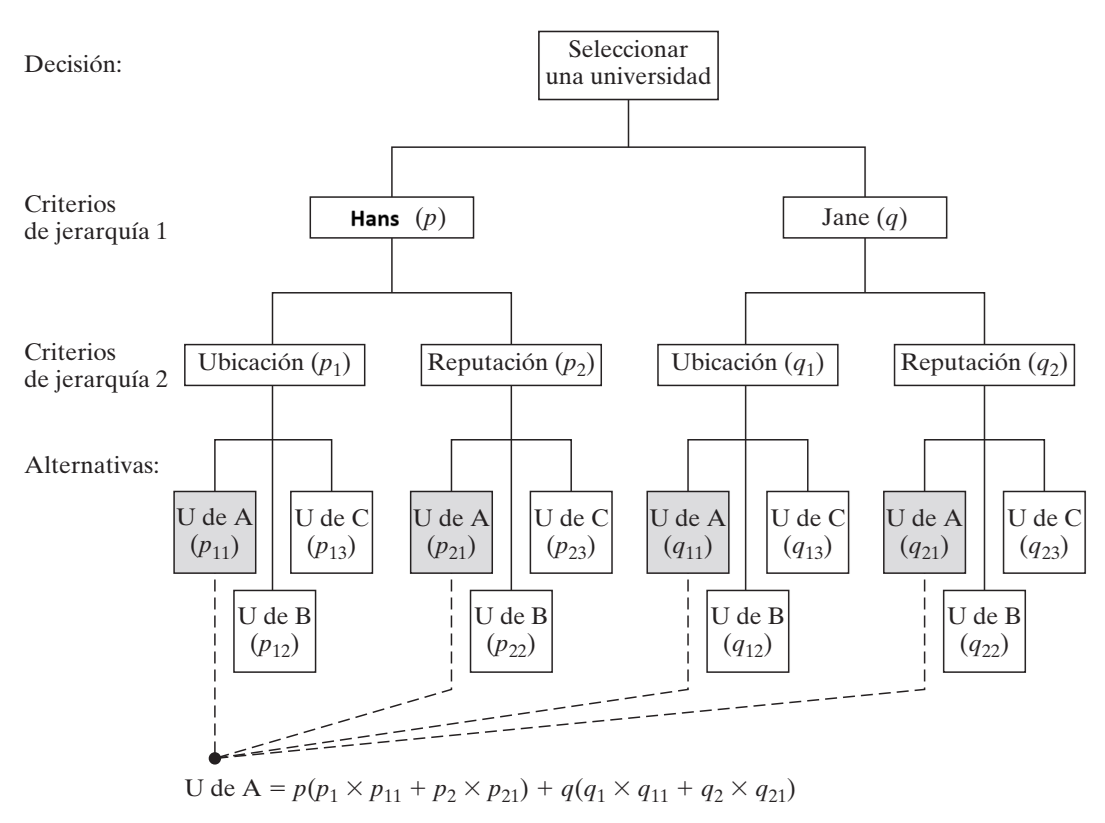
\includegraphics[width=\linewidth]{images/26-decision01.png}
\end{center}
\medskip
En la figura, los pesos relativos de las alternativas respecto de cada criterio se multiplican por los pesos de los criterios, resultando en los pesos compuestos mostrados en la parte inferior.

\subsection*{Peso compuesto de cada universidad}
\begin{align*}
U\;\text{de}\;A&=0.17\times0.129+0.83\times0.545=0.4743,\\
U\;\text{de}\;B&=0.17\times0.277+0.83\times0.273=0.2737,\\
U\;\text{de}\;C&=0.17\times0.594+0.83\times0.182=0.2520.
\end{align*}

\paragraph{Conclusión.} Hans elige la U de A.

Los parámetros $p$ y $q$ representan las preferencias globales de Hans y Jane, respectivamente, sobre los criterios ubicación y reputación. En la segunda jerarquía, los pesos $p_1,p_2$ y $q_1,q_2$ suman 1; lo mismo ocurre con las descomposiciones de alternativas: $p_{11}+p_{12}+p_{13}=1$, etc.

\subsection{Determinación de los pesos}
El quid del PJA es la determinación de pesos relativos. Para $n$ criterios se formula una \textit{matriz de comparación por pares} $A=[a_{ij}]_{n\times n}$, donde $a_{ij}$ mide la importancia de $i$ sobre $j$ con la escala 1–9 de Saaty (1 = igual importancia, 5 = mucho más importante, 9 = extremadamente más importante). La consistencia en el juicio exige $a_{ij}=k\Rightarrow a_{ji}=1/k$ y $a_{ij}a_{jk}=a_{ik}$.

\begin{example}[matriz $A$ para Hans]
Para la jerarquía superior (criterios L y R):
\[A=\begin{pmatrix}1 & 1/5\\ 5 & 1\end{pmatrix}.\]
Normalizando $A$ (dividiendo cada columna por su suma) se obtiene $N$ y los pesos de la fila promediada: $w_L=0.17,\;w_R=0.83$.
\end{example}

Matrices para universidades respecto de L y R:
\[A_L=\begin{pmatrix}1 & 1/2 & 1/5\\ 2 & 1 & 1/2\\ 5 & 2 & 1\end{pmatrix},\quad A_R=\begin{pmatrix}1 & 2 & 3\\ 1/2 & 1 & 3/2\\ 1/3 & 2/3 & 1\end{pmatrix}.\]
Sumas de columna y normalización producen los pesos relativos mostrados en la página anterior.

\subsection*{Razón de consistencia}
Se calcula
\[CI=\frac{\lambda_{\max}-n}{n-1},\quad RI=\frac{1.98(n-2)}{n},\quad CR=\frac{CI}{RI}.\]
Si $CR\le0.10$, la inconsistencia es aceptable.

\newpage
%====================================================
% PÁGINA 517
%====================================================
Al normalizar $A_L$ y $A_R$ se obtienen $N_L$ y $N_R$. Las columnas de $N_R$ son idénticas, por lo que $A_R$ es consistente. Las de $N_L$ difieren, así que $A_L$ no lo es. Para $A_L$ se halla $\lambda_{\max}=3.0113$ y, con $n=3$, resulta $CI=0.00565$, $RI=0.66$, $CR=0.00856$, aceptable al ser $<0.10$.

\newpage
%====================================================
% PÁGINA 518
%====================================================
\section*{Vector de pesos en matrices inconsistentes}
Si $A$ no es consistente, el vector de pesos $\mathbf{w}$ se aproxima por los promedios de fila de la matriz normalizada $N$. Se demuestra que $A\mathbf{w}=\lambda_{\max}\mathbf{w}$ y $\lambda_{\max}\ge n$. Cuanto más se acerque $\lambda_{\max}$ a $n$, más consistente es $A$. Para cuantificar, se define $CI$ y $CR$ como arriba.

\subsection*{Cálculo de $\lambda_{\max}$}
\[\lambda_{\max}=\sum_{i=1}^nw_i^{-1}\Bigl(\sum_{j=1}^na_{ij}w_j\Bigr)w_i.\]

\newpage
%====================================================
% PÁGINA 519
%====================================================
\subsection*{Ejemplo 15.1‑3 (prueba de consistencia de $A_L$)}
Multiplicando $A_L\mathbf{w}$ y sumando los elementos del vector resultante se obtuvo $\lambda_{\max}=3.0113$. Cálculo completo:
\begin{align*}
\lambda_{\max}&=0.3863+0.8320+1.7930=3.0113,\\
CI&=0.00565,\quad RI=0.66,\quad CR=0.00856.
\end{align*}
Al ser $CR<0.10$, el nivel de inconsistencia en $A_L$ es aceptable.

\paragraph{Momento de Excel.} El libro incluye una plantilla \texttt{excelAHP.xlsx} que automatiza los cálculos hasta matrices de 8\,×\,8. Los pesos $w$ se copian a la hoja de resultados, y el proceso se repite con Pegado Especial → Valores para fijar números.

\newpage
%====================================================
% PÁGINA 521
%====================================================
\section*{Problemas adicionales}
\begin{enumerate}[label=\*\arabic*., start=2]
\item El departamento de personal en C\&H busca contratar a Steve (S), Jane (J) o Maisa (M) con criterios entrevista (I), experiencia (E) y referencias (R). Matriz de criterios:
\[A=\begin{pmatrix}1 & 2 & 1/4\\ 1/2 & 1 & 1/3\\ 4 & 5 & 1\end{pmatrix}.\]
Tras entrevistar se generan $A_I, A_E, A_R$ (ver libro). ¿Qué candidato debe ser contratado? Evalúe la consistencia.

\item Kevin y June Park están comprando una casa (A, B, C) y comparan criterios jardinería (Y) y proximidad al trabajo (W). Se suministran $A, A_Y, A_W$. Califique las casas y calcule $CR$.

\item Un nuevo autor escoge editor para un libro (editores H y P) con criterios regalías (R), comercialización (M) y anticipo (A). Se dan $A, A_R, A_M, A_A$. Clasifique y verifique consistencia.
\end{enumerate}

\newpage
%====================================================
% PÁGINA 522
%====================================================
\section*{Problema 5 (elección de mesa directiva)}
Un profesor de ciencias políticas desea predecir el resultado de elección de la mesa directiva. Candidatos Ivy (I), Bahrn (B) y Smith (S). Votantes: izquierda (L), centro (C) y derecha (R). Factores experiencia académica (E), postura ante los problemas (S) y carácter personal (P). Se generan nueve matrices para las jerarquías L, C y R:
\[
A_L=\begin{pmatrix}1 & 2 & 1/2\\ 1/2 & 1 & 1/5\\ 2 & 5 & 1\end{pmatrix},\quad \text{etc.}
\]
El PJA reduce estas matrices a los siguientes pesos relativos:
\begin{table}[H]
\centering
\begin{tabular}{lccc}
\toprule
\textbf{Candidato} & Izquierda & Centro & Derecha\\ \midrule
Ivy & 0.1 & 0.2 & 0.3\\
Bahrn & 0.5 & 0.4 & 0.2\\
Smith & 0.4 & 0.4 & 0.5\\ \bottomrule
\end{tabular}
\end{table}
Determine el ganador y evalúe $CR$.

\section*{Problema 6 (recorte presupuestario escolar)}
El distrito debe reducir gastos: eliminar programa de educación física (E) o música (M). Criterios restricción presupuestaria (B) y necesidades estudiantiles (N). Matrices $A_S$ y $A_P$ como sigue:
\[A_S=\begin{pmatrix}1 & 1\\ 1 & 1\end{pmatrix},\quad A_P=\begin{pmatrix}1 & 1/2\\ 2 & 1\end{pmatrix}.\]

\newpage
%====================================================
% PÁGINA 523
%====================================================
\section*{Problema 7 (compra de automóvil)}
Una persona considera tres modelos de automóvil (M1, M2, M3). Factores: precio de compra (PP), costo de mantenimiento (MC), costo de manejo en ciudad (CD) y en ruta (RD). Datos de costos (3 años de operación):
\begin{table}[H]
\centering
\begin{tabular}{lrrrr}\toprule
\textbf{Modelo} & PP & MC & CD & RD\\ \midrule
M1 & 6\,000 & 1\,800 & 4\,500 & 1\,500\\
M2 & 8\,000 & 1\,200 & 2\,250 & 750\\
M3 & 10\,000 & 600 & 1\,125 & 600\\ \bottomrule
\end{tabular}
\end{table}
Elabore matrices de comparación, evalúe $CR$ y determine el modelo a seleccionar.

\bigskip
\section{Toma de decisiones en condiciones de riesgo}
En condiciones de riesgo, los beneficios asociados con cada alternativa se representan mediante distribuciones de probabilidad y la decisión se basa en el criterio de valor esperado, la maximización de la utilidad esperada o la minimización del costo esperado.

\subsection*{Aplicación de la vida real. Límites en las reservaciones de un hotel}
El hotel La Posada con 300 habitaciones tiene clientes de negocios y de placer. Para maximizar ingresos, fija un límite de reservaciones con descuento para viajeros de placer usando un árbol de decisiones (ver caso 10, capítulo 26).

\subsection{Árbol de decisiones basado en valor esperado}
Considere alternativas $d_i$ y estados de la naturaleza $s_j$ con utilidades $u_{ij}$ y probabilidades $p_j$. El valor esperado es $E[d_i]=\sum_j p_j u_{ij}$.

\end{document}
